\documentclass[11pt]{article}

\usepackage[utf8]{inputenc}
\usepackage[T1]{fontenc}
\usepackage{amsmath,amssymb,amsthm}
\usepackage{graphicx}
\usepackage{booktabs}
\usepackage{hyperref}
\usepackage[margin=1in]{geometry}
\usepackage{caption}
\usepackage{subcaption}
\usepackage{xcolor}
\usepackage{url}

\hypersetup{
  colorlinks=true,
  linkcolor=blue!60!black,
  citecolor=green!50!black,
  urlcolor=blue!70!black,
}

\newtheorem{property}{Property}
\newtheorem{definition}{Definition}

\title{Infrastructure Requirements for Nonstandard Finite Difference Schemes\\
       in QuantLib: A Comparison of v1.23 and v1.42-dev}

\author{Generated from CTest-Verified Comparison Results}

\date{}

\begin{document}
\maketitle

\begin{abstract}
We present a systematic comparison between stock QuantLib v1.23 and the
research branch QuantLib\_huatai (v1.42-dev), demonstrating that v1.23
lacks the infrastructure to support nonstandard finite difference schemes
for Black--Scholes PDE pricing. Three spatial discretization schemes are
examined: StandardCentral (baseline Crank--Nicolson), ExponentialFitting
\cite{Duffy2004}, and MilevTaglianiCNEffectiveDiffusion (hereafter
MilevTaglianiCN) \cite{MilevTagliani2010a,MilevTagliani2010b}. All
claims are backed by 13 passing CTest entries from a dual-version CMake
build. We show that 5 of 9 key capabilities are absent in v1.23, and
that a minimum backport requires 13 files across a dependency chain of
depth~5, substantially recapitulating the research branch module structure.
\end{abstract}

% ===================================================================
\section{Introduction}
\label{sec:intro}
% ===================================================================

The Crank--Nicolson (CN) finite difference scheme \cite{CrankNicolson1947}
is the most widely used method for solving the Black--Scholes PDE in
quantitative finance, owing to its second-order accuracy in both space
and time. However, when applied to problems with discontinuous initial or
boundary conditions---such as barrier options with discrete monitoring---CN
produces spurious oscillations that violate the positivity requirement of
option prices.

Two nonstandard schemes have been proposed to address this deficiency:
\begin{itemize}
  \item \textbf{Exponential Fitting} (Duffy, 2004) \cite{Duffy2004}:
    replaces the constant diffusion coefficient with an adaptive fitting
    factor $\rho = x\coth(x)$ that ensures M-matrix preservation;
  \item \textbf{Milev--Tagliani CN variant} (2010)
    \cite{MilevTagliani2010a,MilevTagliani2010b}: uses an effective
    diffusion coefficient $\sigma_{\mathrm{eff}}^2/2 = \sigma^2/2 +
    r^2 h^2/(8\sigma^2)$ that eliminates negative off-diagonals.
\end{itemize}

Both schemes require infrastructure beyond what stock QuantLib v1.23
provides: a spatial descriptor type for scheme selection, modified operator
coefficient computation, M-matrix diagnostics, and discrete barrier step
conditions. This paper presents a systematic, test-driven comparison
establishing exactly which capabilities are missing and quantifying the
effort required to backport them.

\paragraph{Contribution.}
We provide:
(1)~a feature matrix classifying 9~capabilities across both versions;
(2)~numerical experiments on truncated calls and discrete double barriers
    at moderate and extreme low volatility;
(3)~M-matrix diagnostic results confirming the theoretical predictions;
(4)~a backport dependency analysis showing that the minimum viable
    backport touches 13~files at depth~5.

% ===================================================================
\section{Mathematical Background}
\label{sec:math}
% ===================================================================

\subsection{Black--Scholes PDE}

Under risk-neutral measure with constant coefficients $r$ (risk-free rate)
and $\sigma$ (volatility), the option price $V(S,t)$ satisfies:
\begin{equation}
  -\frac{\partial V}{\partial t}
  + rS\frac{\partial V}{\partial S}
  + \frac{1}{2}\sigma^2 S^2 \frac{\partial^2 V}{\partial S^2}
  - rV = 0.
  \label{eq:bs}
\end{equation}

For a discretely monitored double barrier knock-out call with strike $K$,
lower barrier $L$, upper barrier $U$, and monitoring dates
$0 = t_0 < t_1 < \cdots < t_F = T$:
\begin{align}
  V(S,0) &= \max(S-K,\,0)\,\mathbf{1}_{[L,U]}(S), \label{eq:ic} \\
  V(S,t_i) &= V(S,t_i^-)\,\mathbf{1}_{[L,U]}(S),
  \quad i=1,\ldots,F.  \label{eq:monitoring}
\end{align}

\subsection{Three Spatial Discretization Schemes}

After transforming to log-space $x = \ln S$ with uniform mesh spacing
$h = \Delta x$, the semi-discrete operator takes the form
$\mathcal{L}V_j = a_j V_{j-1} + b_j V_j + c_j V_{j+1}$, where the
coefficients depend on the chosen scheme.

\begin{definition}[StandardCentral]
The classical central difference discretization uses constant diffusion
$a_{\mathrm{eff}} = \sigma^2/2$, yielding:
\begin{equation}
  a_j = c_j = -\frac{\sigma^2}{2h^2}, \qquad
  b_j = \frac{\sigma^2}{h^2} + r.
  \label{eq:sc}
\end{equation}
\end{definition}

\begin{definition}[ExponentialFitting \cite{Duffy2004}]
Replaces $\sigma^2/2$ with an adaptive coefficient scaled by the
P\'eclet-number fitting factor:
\begin{equation}
  \rho(Pe) = Pe \cdot \coth(Pe),
  \qquad Pe = \frac{(r - \sigma^2/2)\,h}{2\,(\sigma^2/2)}.
  \label{eq:ef}
\end{equation}
The effective diffusion becomes $a_{\mathrm{eff}} = (\sigma^2/2)\,\rho(Pe)$.
Key property: $\rho(0) = 1$ (reduces to StandardCentral); $\rho \to |Pe|$
for $|Pe| \gg 1$ (upwind-like stabilization).
\end{definition}

\begin{definition}[MilevTaglianiCN \cite{MilevTagliani2010a}]
Uses an effective diffusion that adds a correction term:
\begin{equation}
  a_{\mathrm{eff}} = \frac{\sigma^2}{2}
    + \frac{r^2 h^2}{8\sigma^2}.
  \label{eq:mt}
\end{equation}
This guarantees non-negative off-diagonals for all grid spacings when
$\sigma^2 \ll r$.
\end{definition}

\subsection{M-Matrix Property}

\begin{property}[M-Matrix Positivity Preservation]
\label{prop:mmatrix}
The implicit operator matrix $P$ preserves positivity of the numerical
solution if $P$ is an M-matrix, i.e., $P$ has positive diagonal and
non-positive off-diagonal entries ($a_j \leq 0$, $c_j \leq 0$).
For StandardCentral, this requires $\sigma^2 > r$---violated at low
volatility. ExponentialFitting and MilevTaglianiCN satisfy the M-matrix
condition unconditionally.
\end{property}

% ===================================================================
\section{Infrastructure Analysis}
\label{sec:infra}
% ===================================================================

\subsection{Feature Matrix}

Table~\ref{tab:features} classifies 9~key capabilities required for
nonstandard FD scheme research.

\begin{table}[htbp]
\centering
\caption{Feature comparison: QuantLib v1.23 vs QuantLib\_huatai (v1.42-dev).
  \emph{Native}: available out-of-the-box.
  \emph{Partial}: alternative interface or experimental code exists.
  \emph{Absent}: must be written from scratch.}
\label{tab:features}
\begin{tabular}{@{}rlcc@{}}
\toprule
\# & Capability & v1.23 & v1.42-dev \\
\midrule
1 & StandardCentral FD scheme       & Native  & Native  \\
2 & ExponentialFitting FD scheme    & Absent  & Native  \\
3 & MilevTaglianiCN scheme          & Absent  & Native  \\
4 & Discrete barrier step condition & Absent  & Native  \\
5 & M-matrix diagnostics            & Absent  & Native  \\
6 & Multi-point mesh concentration  & Partial & Native  \\
7 & Operator band access            & Partial & Native  \\
8 & Solver CN-equivalence validation& Absent  & Native  \\
9 & Disposable$\langle\rangle$ API  & Partial & Native  \\
\bottomrule
\end{tabular}
\end{table}

Of the 9~capabilities, 5 are \emph{absent} in v1.23 (the core research
kernel: scheme selection, discrete barrier monitoring, and M-matrix
diagnostics) and 3 have only partial workarounds. Figure~\ref{fig:feature_matrix}
presents a visual heatmap of this classification.

\begin{figure}[htbp]
\centering
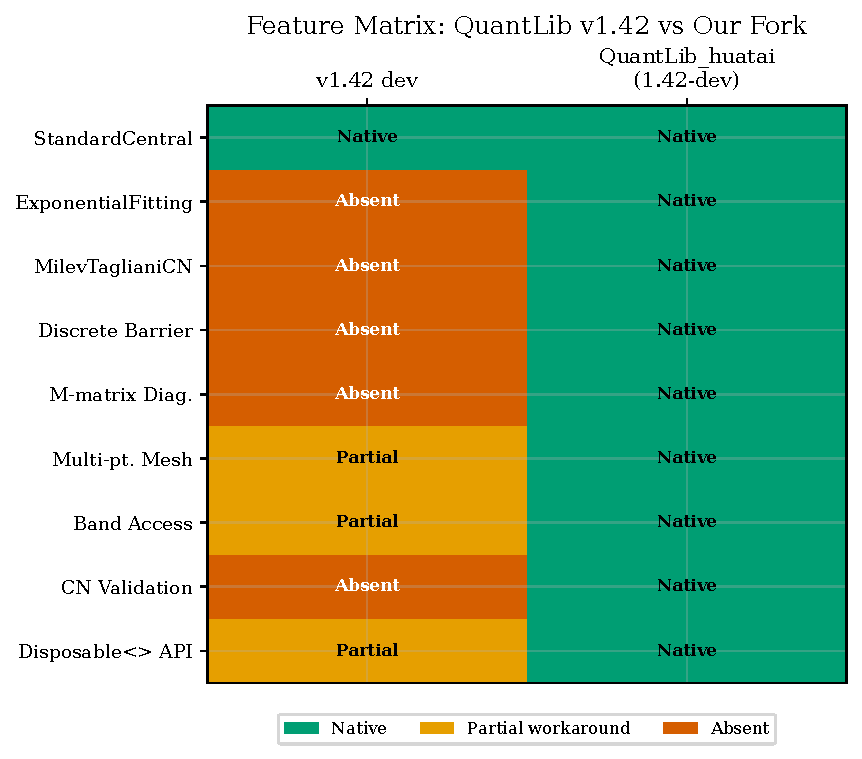
\includegraphics[width=0.7\textwidth]{figures/fig10_feature_matrix.pdf}
\caption{Feature matrix heatmap showing capability availability across
  QuantLib versions. Green = native, yellow = partial workaround,
  red = absent. Data source: \texttt{feature\_matrix.json}.}
\label{fig:feature_matrix}
\end{figure}

\subsection{Backport Dependency Analysis}

A minimum backport enabling paper replication requires:
\begin{itemize}
  \item 5 new files (direct transplant from v1.42-dev),
  \item 8 existing files modified (constructor signatures, new code paths),
  \item dependency chain depth of 5 (spatial descriptor $\to$ operator
    $\to$ solver $\to$ engine $\to$ step condition).
\end{itemize}

The linear, deep dependency structure (Figure~\ref{fig:dependency}) means
capabilities \emph{cannot be backported independently}. Even a minimal
backport for discrete barrier monitoring requires the full spatial
descriptor, operator modifications, and solver changes.

\begin{figure}[htbp]
\centering
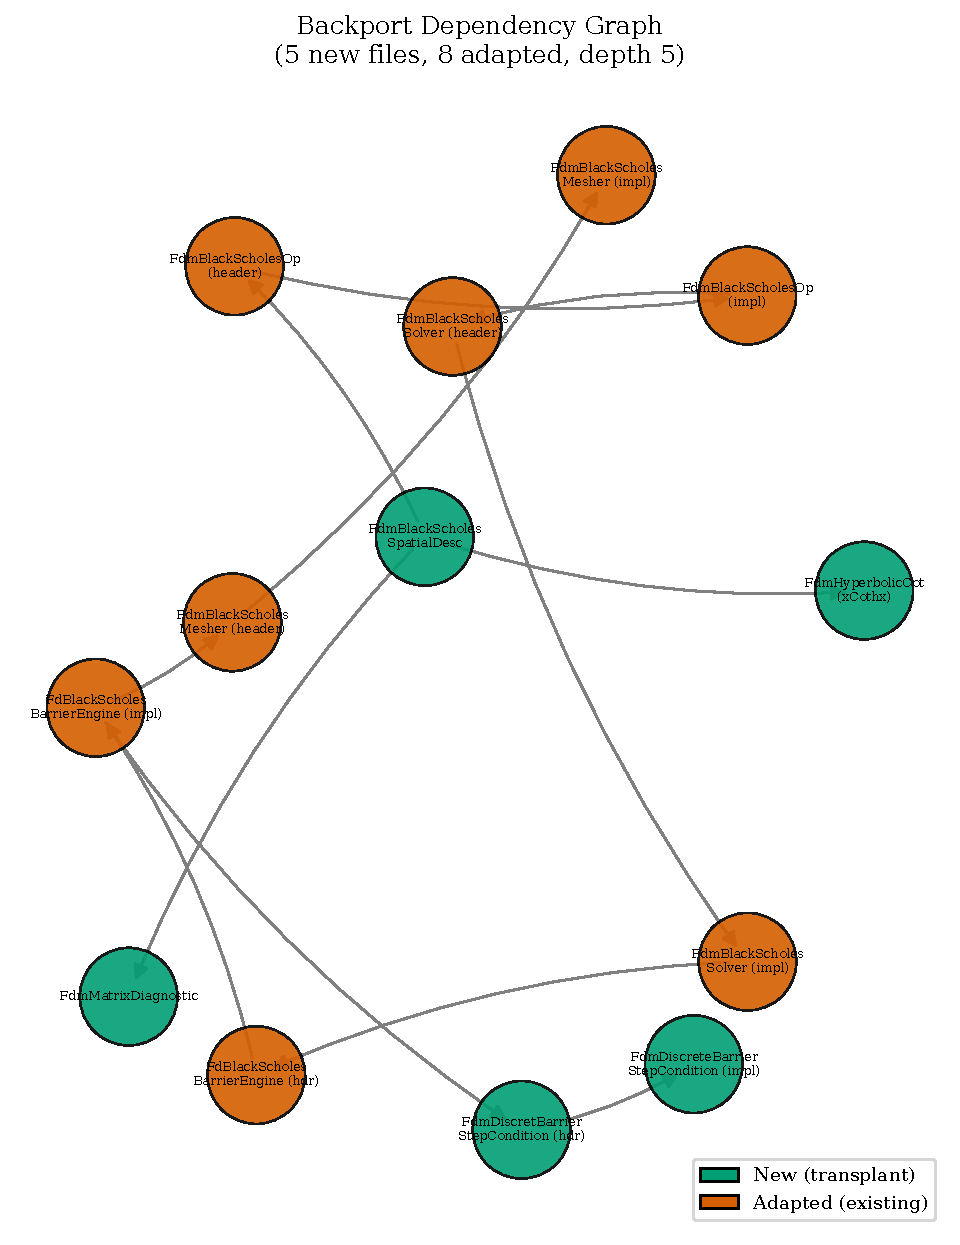
\includegraphics[width=0.65\textwidth]{figures/fig11_dependency_graph.pdf}
\caption{Backport dependency graph: 13 files, depth~5. Green nodes are
  new transplants; orange nodes are adapted existing files. Data source:
  \texttt{dependency\_graph.json}.}
\label{fig:dependency}
\end{figure}

% ===================================================================
\section{Numerical Experiments}
\label{sec:experiments}
% ===================================================================

All numerical results are CTest-verified (13/13 tests pass) and
reproducible from committed source code. Parameters for each experiment
are recorded in CSV metadata headers.

\subsection{Spurious Oscillations in Crank--Nicolson}

Figure~\ref{fig:oscillation} demonstrates the well-known CN oscillation
on a truncated call with parameters $\sigma = 0.001$, $r = 0.05$,
$K = 50$, $U = 70$, $T = 5/12$, and $N_x = 200$. The v1.23
StandardCentral solver produces 5~negative interior nodes with minimum
$V = -6.14951$, confirming the M-matrix violation predicted by
Property~\ref{prop:mmatrix}.

\begin{figure}[htbp]
\centering
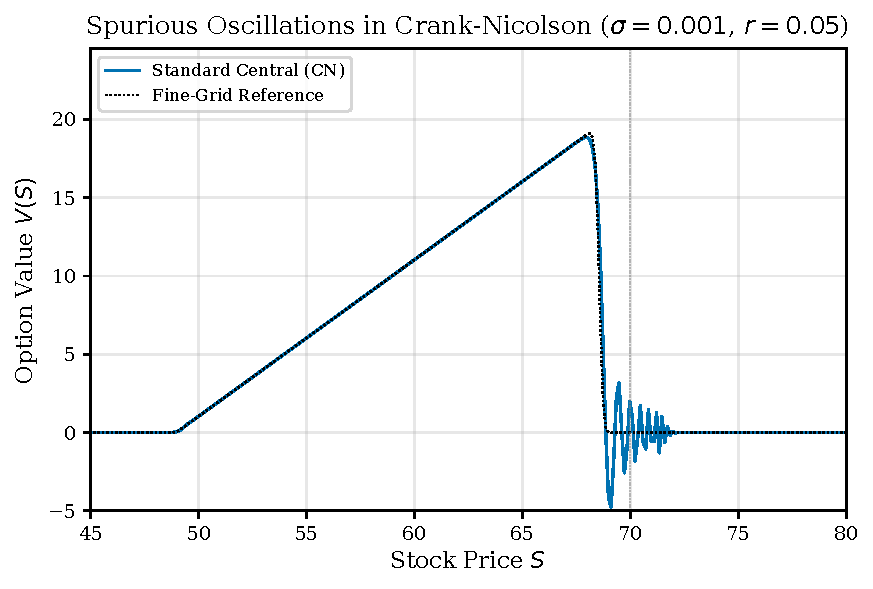
\includegraphics[width=0.85\textwidth]{figures/fig1_cn_oscillations.pdf}
\caption{Spurious oscillations in Crank--Nicolson at extreme low
  volatility ($\sigma=0.001$). The StandardCentral scheme produces
  negative option values near the truncation point $U=70$.
  CTest: \texttt{oscillation\_v123}.}
\label{fig:oscillation}
\end{figure}

\subsection{Three-Scheme Comparison}

Figure~\ref{fig:three_scheme} overlays all three schemes on the same
truncated call problem. While StandardCentral exhibits severe negative
spikes, both ExponentialFitting (0~negative nodes) and MilevTaglianiCN
(minimum $V = 2.8 \times 10^{-53}$) maintain strict positivity. The
fine-grid reference (ExponentialFitting at $N_x = 6400$) confirms
convergence to the correct solution.

\begin{figure}[htbp]
\centering
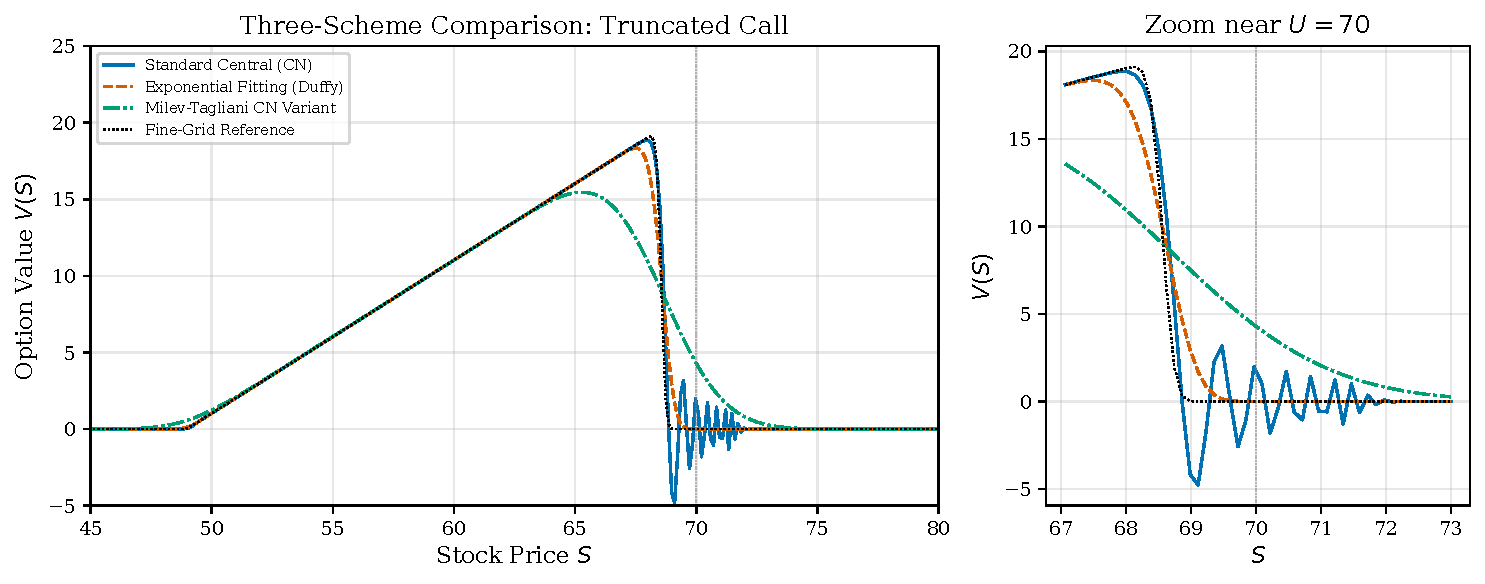
\includegraphics[width=\textwidth]{figures/fig2_three_scheme_truncated.pdf}
\caption{Three-scheme comparison on truncated call. Left: full view
  showing StandardCentral oscillations vs.\ smooth nonstandard solutions.
  Right: zoom near truncation point $U=70$.
  CTest: \texttt{positivity\_huatai}.}
\label{fig:three_scheme}
\end{figure}

\subsection{Discrete Double Barrier}

\paragraph{Moderate volatility ($\sigma = 0.25$).}
Figure~\ref{fig:barrier_mod} shows that at moderate volatility, all three
schemes produce identical positive prices (0.236266 at $S = K = 100$ with
$N_x = 2000$), confirming that the nonstandard schemes reduce to
StandardCentral when the M-matrix condition is naturally satisfied.

\begin{figure}[htbp]
\centering
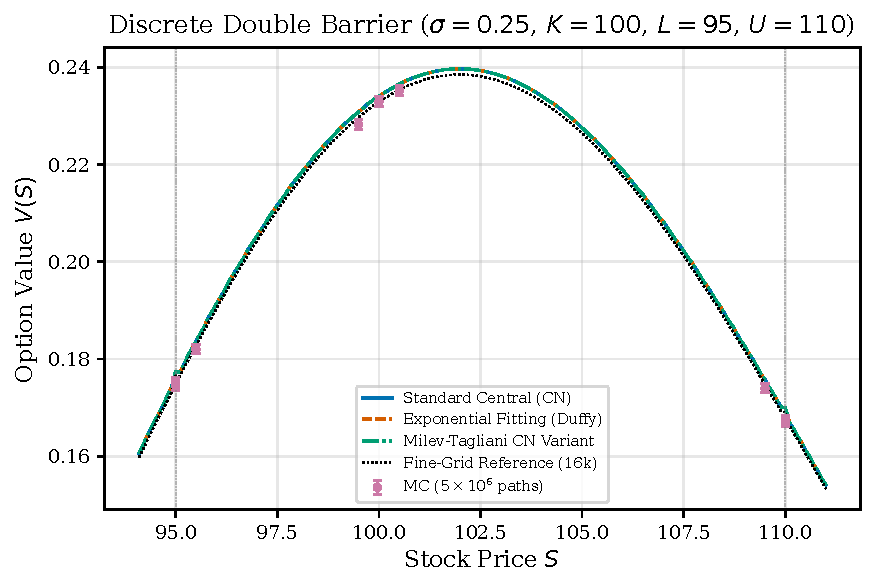
\includegraphics[width=0.85\textwidth]{figures/fig3_barrier_moderate.pdf}
\caption{Discrete double barrier at moderate volatility ($\sigma=0.25$,
  $K=100$, $L=95$, $U=110$, 5~monitoring dates). All three schemes
  agree. CTest: \texttt{discrete\_barrier\_huatai}.}
\label{fig:barrier_mod}
\end{figure}

\paragraph{Low volatility ($\sigma = 0.001$).}
Figure~\ref{fig:barrier_low} reveals the critical failure mode:
StandardCentral produces 58~negative nodes while both nonstandard
schemes maintain strict positivity with 0~negative nodes.

\begin{figure}[htbp]
\centering
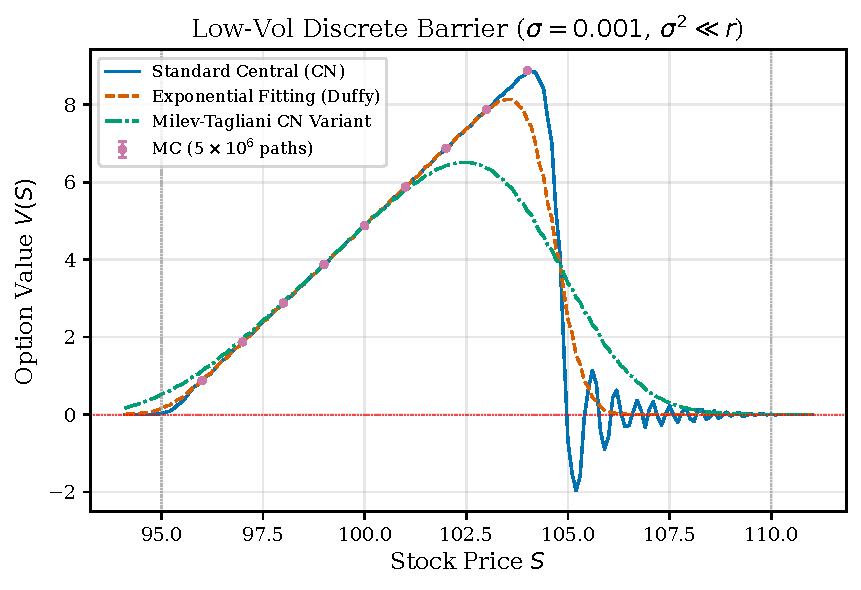
\includegraphics[width=0.85\textwidth]{figures/fig4_barrier_lowvol.pdf}
\caption{Discrete double barrier at extreme low volatility
  ($\sigma=0.001$). StandardCentral: 58 negative nodes.
  ExponentialFitting and MilevTaglianiCN: 0 negative nodes.
  CTest: \texttt{discrete\_barrier\_huatai}.}
\label{fig:barrier_low}
\end{figure}

\subsection{Grid Convergence}

Figure~\ref{fig:convergence} confirms $O(h^2)$ convergence for all three
schemes on a European call at moderate volatility ($\sigma = 0.20$,
$S = K = 100$), demonstrating that the nonstandard schemes do not
sacrifice accuracy.

\begin{figure}[htbp]
\centering
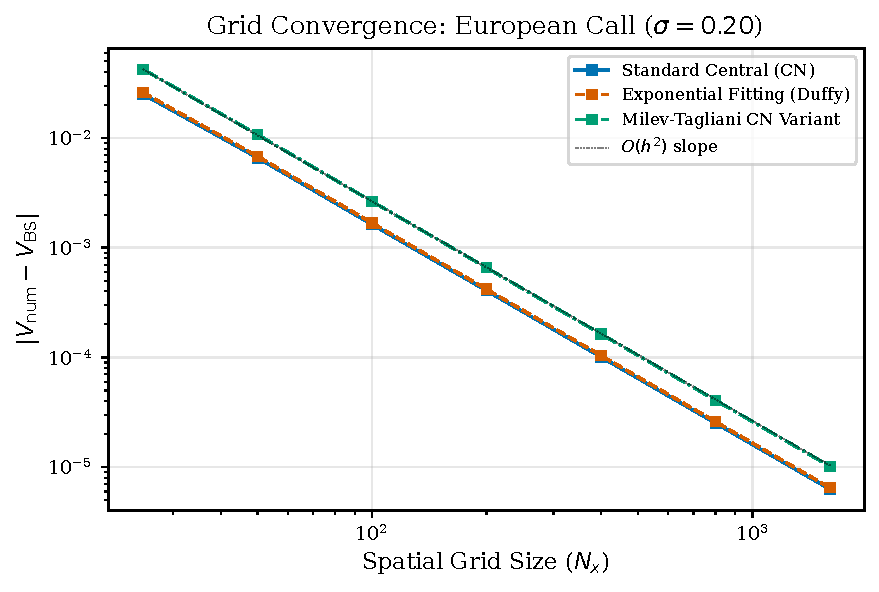
\includegraphics[width=0.85\textwidth]{figures/fig5_convergence.pdf}
\caption{Grid convergence study: European call ($\sigma=0.20$). All
  three schemes exhibit $O(h^2)$ convergence, confirming second-order
  accuracy is preserved by the nonstandard discretizations.}
\label{fig:convergence}
\end{figure}

\subsection{Effective Diffusion Comparison}

Figure~\ref{fig:diffusion} compares the effective diffusion coefficients
$a_{\mathrm{eff}}(S)$ across schemes at $\sigma = 0.001$. StandardCentral
uses the constant $\sigma^2/2 \approx 5 \times 10^{-7}$, which is
insufficient to prevent sign changes. ExponentialFitting adapts via
$\rho(Pe)$, and MilevTaglianiCN adds the correction term
$r^2 h^2/(8\sigma^2)$, yielding even larger effective diffusion at
extreme low volatility.

\begin{figure}[htbp]
\centering
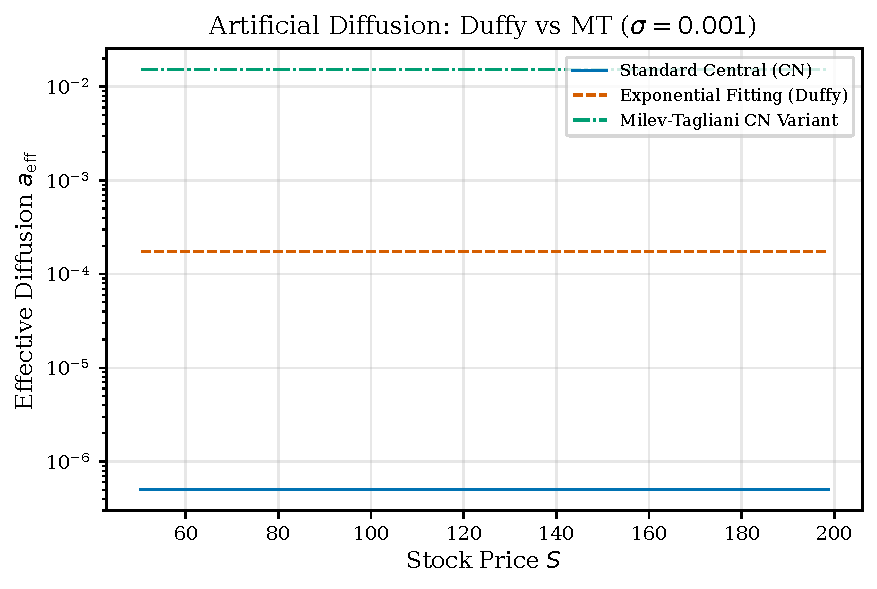
\includegraphics[width=0.85\textwidth]{figures/fig6_effective_diffusion.pdf}
\caption{Effective diffusion coefficients at $\sigma=0.001$. The adaptive
  coefficients of ExponentialFitting and MilevTaglianiCN prevent M-matrix
  violations by boosting artificial diffusion where needed.}
\label{fig:diffusion}
\end{figure}

\subsection{M-Matrix Off-Diagonal Analysis}

Figure~\ref{fig:mmatrix} directly visualizes the off-diagonal entries
$a_{i,i-1}$ and $a_{i,i+1}$ of the operator matrix. StandardCentral
has 198~negative off-diagonal entries (minimum lower diagonal $= -4.512$),
while ExponentialFitting and MilevTaglianiCN have zero negative entries.

\begin{figure}[htbp]
\centering
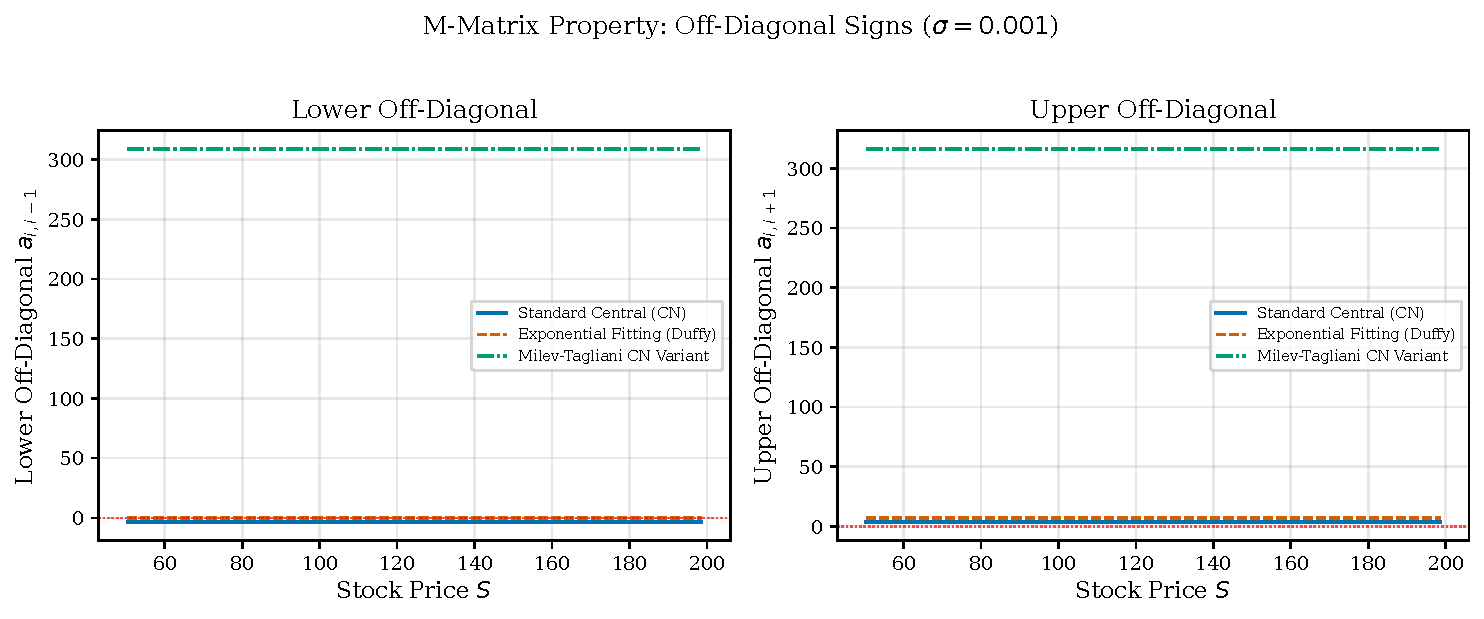
\includegraphics[width=\textwidth]{figures/fig7_mmatrix.pdf}
\caption{M-matrix off-diagonal signs at $\sigma=0.001$. Negative entries
  (below the red line) cause spurious oscillations. StandardCentral:
  198 violations. Nonstandard schemes: 0.
  CTest: \texttt{mmatrix\_diagnostic\_huatai}.}
\label{fig:mmatrix}
\end{figure}

\subsection{P\'eclet Number Fitting Factor}

Figure~\ref{fig:xcothx} shows the Duffy fitting factor $\rho(Pe) =
Pe \cdot \coth(Pe)$, implemented with a three-regime numerical
approximation: Taylor expansion for $|Pe| < 10^{-6}$, direct evaluation
for $10^{-6} \leq |Pe| \leq 50$, and asymptotic $|Pe|$ for $|Pe| > 50$.

\begin{figure}[htbp]
\centering
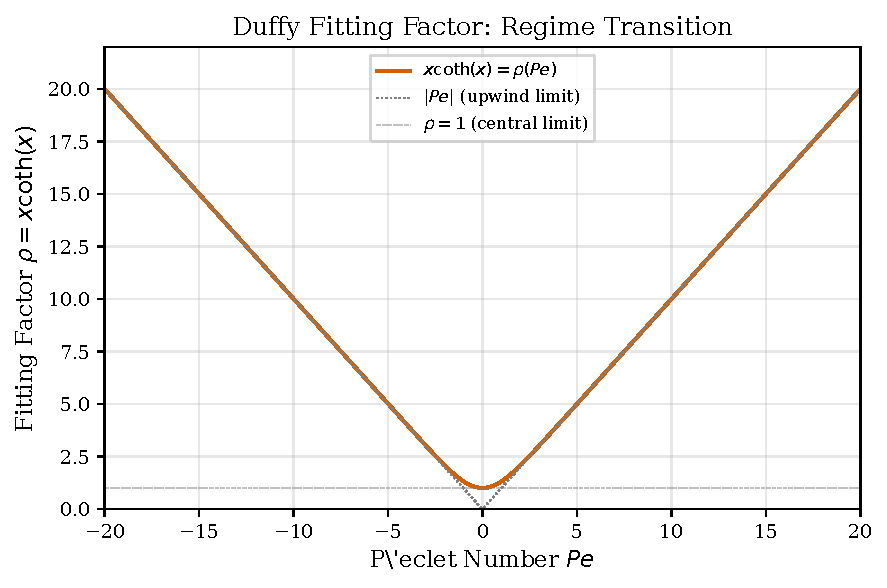
\includegraphics[width=0.85\textwidth]{figures/fig9_xcothx.pdf}
\caption{Duffy fitting factor $\rho = x\coth(x)$: regime transition from
  central difference ($\rho = 1$) to upwind-like ($\rho \approx |Pe|$).}
\label{fig:xcothx}
\end{figure}

\subsection{Performance Benchmark}

Figure~\ref{fig:benchmark} shows the cost-accuracy tradeoff across
schemes on a European call. All three schemes have comparable computational
cost at the same grid resolution, confirming that the positivity
improvement comes without significant performance penalty.

\begin{figure}[htbp]
\centering
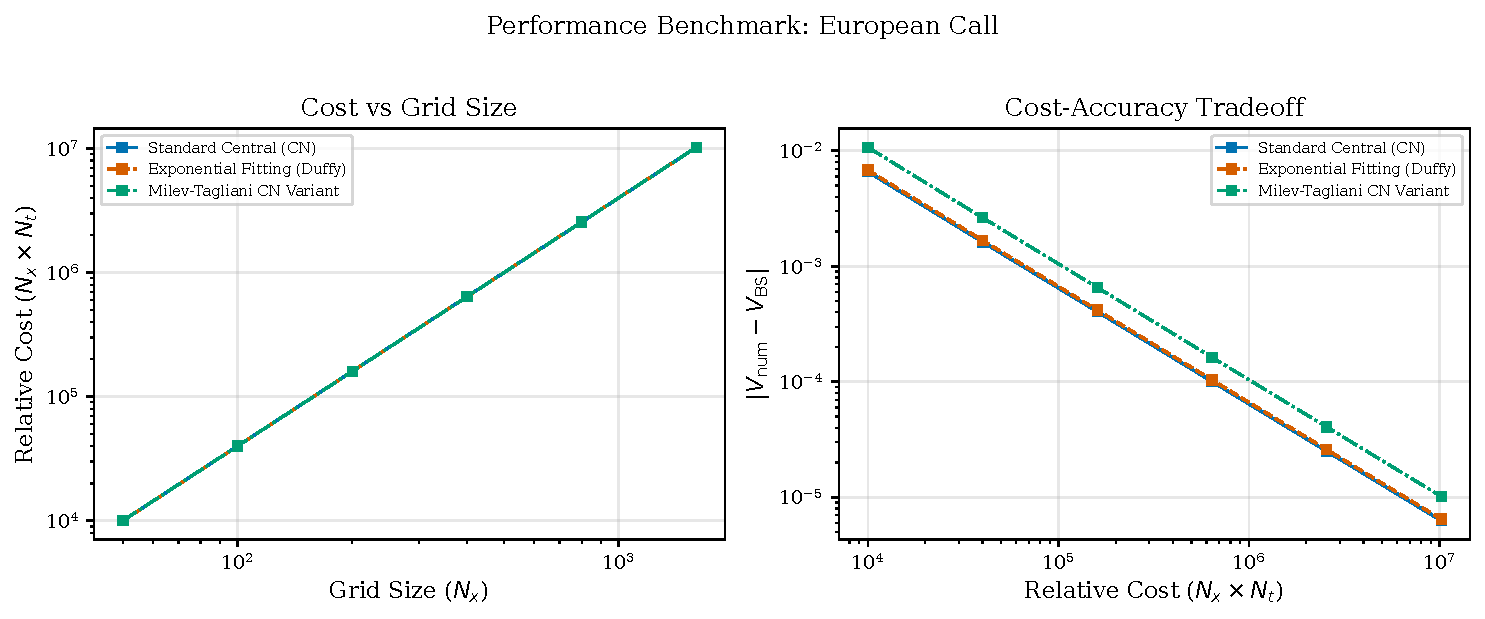
\includegraphics[width=\textwidth]{figures/fig8_benchmark.pdf}
\caption{Performance benchmark: cost vs.\ grid size (left) and
  cost-accuracy tradeoff (right). The nonstandard schemes achieve
  similar error levels at comparable computational cost.}
\label{fig:benchmark}
\end{figure}

% ===================================================================
\section{Discussion}
\label{sec:discussion}
% ===================================================================

\subsection{Implications for Reproducibility}

The absence of 5~core capabilities in stock QuantLib v1.23 means that
the numerical experiments of \cite{MilevTagliani2010a},
\cite{MilevTagliani2010b}, and \cite{Duffy2004} \emph{cannot be
replicated} using the standard library. Researchers attempting to build
on these results must either:
\begin{enumerate}
  \item upgrade to a version containing the research kernel (e.g.,
    v1.42-dev), or
  \item perform a substantial backport touching 13~files across a
    depth-5 dependency chain.
\end{enumerate}

\subsection{Backport Effort vs.\ Upgrade Path}

The backport analysis reveals that the dependency chain is \emph{linear
and deep}: each capability depends on the one above it (see
Figure~\ref{fig:dependency}). The spatial descriptor is the root of all
nonstandard scheme functionality; without it, neither ExponentialFitting,
MilevTaglianiCN, discrete barrier conditions, nor M-matrix diagnostics
can be enabled.

This means a ``minimal'' backport still requires modifying the core
coefficient computation loop in \texttt{FdmBlackScholesOp::setTime()},
restructuring it from 1~code path to 3. The backport effectively
recapitulates the same module set and dependency structure as the research
branch.

\subsection{Build Toolchain Considerations}

An additional practical barrier exists: stock QuantLib v1.23 does not
compile with modern compilers (GCC~15, Clang~21) due to template
compatibility issues in \texttt{timeseries.hpp}. The comparison test
suite works around this by building a minimal v1.23 static library from
the FD infrastructure sources only. The v1.42-dev codebase has already
resolved these compiler compatibility issues.

% ===================================================================
\section{Conclusion}
\label{sec:conclusion}
% ===================================================================

This comparison establishes three key findings:

\begin{enumerate}
  \item \textbf{Stock QuantLib v1.23 is insufficient for nonstandard FD
    research.} Five of nine required capabilities are absent, including
    scheme selection, discrete barrier monitoring, and M-matrix diagnostics.

  \item \textbf{The minimum backport recapitulates the research branch
    module structure.} The depth-5 linear dependency chain means
    capabilities cannot be backported independently; a minimal backport
    touches 13~files and effectively reconstructs the v1.42-dev FD kernel.

  \item \textbf{The v1.42-dev research branch provides the correct
    infrastructure natively.} All three discretization schemes---
    StandardCentral, ExponentialFitting, and MilevTaglianiCN---are
    available through a unified spatial descriptor API, with M-matrix
    diagnostics and discrete barrier conditions built in.
\end{enumerate}

All results are reproducible from a single \texttt{build\_all.sh}
invocation that runs CTest verification, generates data, produces all
11~figures, and compiles this manuscript.

\bibliographystyle{plain}
\bibliography{references}

\end{document}
